%%%%%%%%%%%%%%%%%%%%%%%%%%%%%%%%%%%%%%%%%
% Masters/Doctoral Thesis 
% LaTeX Template
% Version 2.5 (27/8/17)
%
% This template was downloaded from:
% http://www.LaTeXTemplates.com
%
% Version 2.x major modifications by:
% Vel (vel@latextemplates.com)
%
% This template is based on a template by:
% Steve Gunn (http://users.ecs.soton.ac.uk/srg/softwaretools/document/templates/)
% Sunil Patel (http://www.sunilpatel.co.uk/thesis-template/)
%
% Template license:
% CC BY-NC-SA 3.0 (http://creativecommons.org/licenses/by-nc-sa/3.0/)
%
%%%%%%%%%%%%%%%%%%%%%%%%%%%%%%%%%%%%%%%%%

%----------------------------------------------------------------------------------------
%	PACKAGES AND OTHER DOCUMENT CONFIGURATIONS
%----------------------------------------------------------------------------------------

\documentclass[
11pt, % The default document font size, options: 10pt, 11pt, 12pt
%oneside, % Two side (alternating margins) for binding by default, uncomment to switch to one side
spanish, % ngerman for German
singlespacing, % Single line spacing, alternatives: onehalfspacing or doublespacing
%draft, % Uncomment to enable draft mode (no pictures, no links, overfull hboxes indicated)
%nolistspacing, % If the document is onehalfspacing or doublespacing, uncomment this to set spacing in lists to single
%liststotoc, % Uncomment to add the list of figures/tables/etc to the table of contents
%toctotoc, % Uncomment to add the main table of contents to the table of contents
%parskip, % Uncomment to add space between paragraphs
%nohyperref, % Uncomment to not load the hyperref package
headsepline, % Uncomment to get a line under the header
%chapterinoneline, % Uncomment to place the chapter title next to the number on one line
%consistentlayout, % Uncomment to change the layout of the declaration, abstract and acknowledgements pages to match the default layout
]{MastersDoctoralThesis} % The class file specifying the document structure

\usepackage[utf8]{inputenc} % Required for inputting international characters
\usepackage[T1]{fontenc} % Output font encoding for international characters
\usepackage{subcaption}
\usepackage{enumerate}

\usepackage{mathpazo} % Use the Palatino font by default

\usepackage[backend=bibtex,style=authoryear,natbib=true]{biblatex} % Use the bibtex backend with the authoryear citation style (which resembles APA)

\addbibresource{references.bib} % The filename of the bibliography

\usepackage[autostyle=true]{csquotes} % Required to generate language-dependent quotes in the bibliography

%----------------------------------------------------------------------------------------
%	MARGIN SETTINGS
%----------------------------------------------------------------------------------------

\geometry{
	paper=a4paper, % Change to letterpaper for US letter
	inner=2.5cm, % Inner margin
	outer=3.8cm, % Outer margin
	bindingoffset=.5cm, % Binding offset
	top=1.5cm, % Top margin
	bottom=1.5cm, % Bottom margin
	%showframe, % Uncomment to show how the type block is set on the page
}

%----------------------------------------------------------------------------------------
%	THESIS INFORMATION
%----------------------------------------------------------------------------------------

\thesistitle{ Estudio del \textit{``Impossible Early Galaxy Problem''} y sus posibles soluciones.} % Your thesis title, this is used in the title and abstract, print it elsewhere with \ttitle
\supervisor{Dr. Santi \textsc{Roca Fabrega}} % Your supervisor's name, this is used in the title page, print it elsewhere with \supname
\examiner{} % Your examiner's name, this is not currently used anywhere in the template, print it elsewhere with \examname
\degree{Máster universitario en Astrofísica} % Your degree name, this is used in the title page and abstract, print it elsewhere with \degreename
\author{Santiago \textsc{Arranz Sanz}} % Your name, this is used in the title page and abstract, print it elsewhere with \authorname
\addresses{} % Your address, this is not currently used anywhere in the template, print it elsewhere with \addressname

\subject{Ciencias Físicas} % Your subject area, this is not currently used anywhere in the template, print it elsewhere with \subjectname
\keywords{} % Keywords for your thesis, this is not currently used anywhere in the template, print it elsewhere with \keywordnames
\university{\href{https://www.ucm.es/}{Universidad Complutense de Madrid}} % Your university's name and URL, this is used in the title page and abstract, print it elsewhere with \univname
\department{\href{https://webs.ucm.es/info/Astrof/}{Departmento de Astrofísica}} % Your department's name and URL, this is used in the title page and abstract, print it elsewhere with \deptname
\group{\href{http://researchgroup.university.com}{Research Group Name}} % Your research group's name and URL, this is used in the title page, print it elsewhere with \groupname
\faculty{\href{https://fisicas.ucm.es/}{Facultad de Ciencias Físicas}} % Your faculty's name and URL, this is used in the title page and abstract, print it elsewhere with \facname

\AtBeginDocument{
\hypersetup{pdftitle=\ttitle} % Set the PDF's title to your title
\hypersetup{pdfauthor=\authorname} % Set the PDF's author to your name
\hypersetup{pdfkeywords=\keywordnames} % Set the PDF's keywords to your keywords
}

\begin{document}

\frontmatter % Use roman page numbering style (i, ii, iii, iv...) for the pre-content pages

\pagestyle{plain} % Default to the plain heading style until the thesis style is called for the body content

%----------------------------------------------------------------------------------------
%	TITLE PAGE
%----------------------------------------------------------------------------------------

\begin{titlepage}
\begin{center}

\vspace*{.06\textheight}
{\scshape\LARGE \univname\par}\vspace{1.5cm} % University name
\textsc{\Large Trabajo Fin de Máster}\\[0.5cm] % Thesis type

\HRule \\[0.4cm] % Horizontal line
{\huge \bfseries \ttitle\par}\vspace{0.4cm} % Thesis title
\HRule \\[1.5cm] % Horizontal line
 
\begin{minipage}[t]{0.4\textwidth}
\begin{flushleft} \large
\emph{Autor:}\\
\href{}{\authorname} % Author name - remove the \href bracket to remove the link
\end{flushleft}
\end{minipage}
\begin{minipage}[t]{0.4\textwidth}
\begin{flushright} \large
\emph{Tutor:} \\
\href{https://fisicas.ucm.es/directorio?id=30649}{\supname} % Supervisor name - remove the \href bracket to remove the link  
\end{flushright}
\end{minipage}\\[3cm]
 
\vfill

\large \textit{Un trabajo requerido para completar\\ el \degreename}\\[0.3cm] % University requirement text
\textit{in the}\\[0.4cm]
\deptname\\[2cm] % Research group name and department name
 
\vfill

{\large \today}\\[4cm] % Date
%\includegraphics{Logo} % University/department logo - uncomment to place it
 
\vfill
\end{center}
\end{titlepage}

%----------------------------------------------------------------------------------------
%	CITA, AGRADECIMIENTOS Y DEDICATORIA
%----------------------------------------------------------------------------------------
%%----------------------------------------------------------------------------------------
%	DEDICATION
%----------------------------------------------------------------------------------------

\dedicatory{En memoría y honor de mi padre.} 

%----------------------------------------------------------------------------------------
%	QUOTATION PAGE
%----------------------------------------------------------------------------------------

\cleardoublepage
\vspace*{0.2\textheight}

\noindent\enquote{\itshape Los pioneros siembran y sus hijos recogen.}\bigbreak

\hfill Ignacio Arranz Sanz.

%----------------------------------------------------------------------------------------
%	ACKNOWLEDGEMENTS
%----------------------------------------------------------------------------------------

\begin{acknowledgements}
\addchaptertocentry{\acknowledgementname} % Add the acknowledgements to the table of contents
Gracias a la paciencia y tiemp de mi tutor.\ldots
\end{acknowledgements}

%----------------------------------------------------------------------------------------
%	ABSTRACT PAGE
%----------------------------------------------------------------------------------------

\begin{abstract}
\addchaptertocentry{\newabstractname} % Add the abstract to the table of contents
El trabajo intenta abordar la problemática surgida en el paper de \cite{steinhardt2016impossibly}, denominado por los autores como \textit{``The Impossible Early Galaxy Problem''}, desde el punto de vista observacional, del modelo de cecimiento de las galaxias y del modelo cosmológico adoptado. Por último se esbozará las posibles soluciones encontradas por otros autores y se marcarán posibles vías de investigación para profundizar en posibles futuros trabajos.
\end{abstract}



%----------------------------------------------------------------------------------------
%	THESIS CONTENT - CHAPTERS
%----------------------------------------------------------------------------------------

\mainmatter % Begin numeric (1,2,3...) page numbering

\pagestyle{thesis} % Return the page headers back to the "thesis" style

% Include the chapters of the thesis as separate files from the Chapters folder
% Uncomment the lines as you write the chapters
% Chapter 1 v2

\chapter{Luces y sombras del modelo cosmológico estándar} % Main chapter title

\label{introduction} % For referencing the chapter elsewhere, use \ref{Chapter1} 

%----------------------------------------------------------------------------------------

% Define some commands to keep the formatting separated from the content 
\newcommand{\keyword}[1]{\textbf{#1}}
\newcommand{\tabhead}[1]{\textbf{#1}}
\newcommand{\code}[1]{\texttt{#1}}
\newcommand{\file}[1]{\texttt{\bfseries#1}}
\newcommand{\option}[1]{\texttt{\itshape#1}}
\newcommand{\lcdm}{$\Lambda$CDM }
\newcommand{\addcite}{\textcolor{red}{[CITA]}}

%----------------------------------------------------------------------------------------

\section{Modelo cosmológico estándar, breve descripción y principales logros.}
Dentro del modelo cosmológico estándar \lcdm, el cual queda restringido al marco de la relatividad general de Einstein con una componentes de energía oscura correspondiente a un fluido con parámetro de estado de $\omega=-1$ y a una 
naturaleza fría de la materia oscura denominada \textit{Cold Dark Matter}, existe un gran consenso en la teoría de la formación y evolución de estructuras del Universo \addcite, siendo su origen las fluctuaciones cuánticas que dejo a descubierto el rápido proceso de inflacción ocurrido pocos \textcolor{red}{nano segundos} después del Big Bang y que crecieron en una primera fase de manera lineal producto de procesos de autoalimentación de las fluctuaciones existente \addcite, sin embargo existe un límite donde esa descripción es validad y entran en una fase de crecimiento no lineal. Es en este punto donde el avance de las últimas décadas ha arrojado más luz, sirviéndose de simulaciones de N-cuerpos cada vez más depurados (Millenium, Bolshoi,...)\addcite que nos permite ver como se acumula la materia oscura y modelos semi-analíticos (de Lucia,...)\addcite donde se añaden las recetas de la física bariónica, nos permiten simular escenarios hasta el universo local pudiendo ver desde las estadísticas de grandes números \addcite hasta las características de rotación de las galaxias espirales en $z\sim 0$ \addcite.\\

En el contexto de este paradigma de modelo estándar más un modelo jerárquico de evolución de galaxias, donde se considera que la evolución de las éstas parte de pequeñas galaxias que van sufriendo diversas fusiones con otras galaxias a lo largo de su vida hasta llegar formar grandes galaxias, agrupándose en grandes cúmulos \addcite .Algunas de las predicciones o grandes logros del modelo cosmológico pueden ser la detección del fondo cósmico de microondas a una temperatura de $3^\circ\mathrm{K}$ \addcite, la abundacia de elementos ligeros como el deuterio $D$, el helio tres $3^He$, la fracción de helio cuatro $4^He/H\sim 0.25$ y del litio siete $7^Li$ \addcite , la precisión de los parámetros cosmológicos deducidos por la teoría y observados como la fracción bariónica $\Omega_b$, la abundacnia de neutrinos y fotones, la precisión en el parámetro de expansión del universo y aceleración, etc \addcite.\\

Procesos como la observación de una gran abundancia de galaxias del tipo \textit{``temprano''} \footnote{El termino temprano está traducido del término ``\textit{earl-type}'' en ingles en donde hace referencia a las galaxias principalmente del tipo elíptico, ya que en época de Hubble se consideraban las galaxias evolucionabas de elipticas a espirales las cuales se denotaban como del tipo \textit{``tardío''} o en inglés \textit{``old-type''}, cosa que se demostró no ser cierta siendo precisamente una prueba que en épocas de $z\sim 2$ la abundancia de galaxias del tipo elíptico eran mucho menos abundantes que en la actualidad.} en el Universo local mientras que en épocas $z >2$ su abundancia es mucho menos notoria observándose una mayor cantidad de galaxias del tipo \textit{``tardío''} \addcite respaldan el modelo jerárquicos de evolución de galaxias \addcite. Otras de éstas observaciones es la abundancia de galaxias satélites (con respecto a otros modelos de materia oscura),......



\section{Naturaleza de la materia oscura, teorías y principales ventajas y desventajas de estás}

\section{Evolución jerárquica de galaxias en la cosmología estándar.}

\subsection{Descripción y teoría.}
\subsection{Simulaciones.}
\subsection{Predicciones, Problemas y Observaciones. Hasta que punto esos problemas se pueden solucionar en el modelo estándar.}

\section{ El papel actual de la física barionica como héroe al rescate a los problemas de la cosmología estándar.}

\section{Papel de los modelos cosmológicos ante los mismos problemas y observaciones.}

\section{¿En qué punto nos encontramos? ¿Por qué no encontramos candidatos a la CDM? Resumen.}


%% Chapter 1

\chapter{Introducción} % Main chapter title

\label{introduction} % For referencing the chapter elsewhere, use \ref{Chapter1} 

%----------------------------------------------------------------------------------------

% Define some commands to keep the formatting separated from the content 
\newcommand{\keyword}[1]{\textbf{#1}}
\newcommand{\tabhead}[1]{\textbf{#1}}
\newcommand{\code}[1]{\texttt{#1}}
\newcommand{\file}[1]{\texttt{\bfseries#1}}
\newcommand{\option}[1]{\texttt{\itshape#1}}
\newcommand{\lcdm}{$\Lambda$CDM }

%----------------------------------------------------------------------------------------


El origen de este trabajo iba a ser el estudio del modelo de crecimiento de galaxias bajo la influencia por una naturaleza \textit{warm dark matter} (WDM), en contraposición al modelo estandar asociado a la \textit{cold dark matter} (CDM). La finalidad era el estudio de la simulaciones de WDM pero debido al escaso cat\'alogo de estas simulaciones y el estatus de este trabajo se opt\'o por otro enfoque. Dicho enfoque pas\'o desde una perspectiva centrada a las simulaciones num\'ericas a un visi\'on m\'as te\'orica con la esperanza de poder ser traducida en un fut\'uro a una estado m\'as pr\'actica.\\

El objeto de este trabajo es el \textit{Impossible Early Galaxy Problem} (IEGP), definido por primera vez en el \textit{paper} \cite{steinhardt2016impossibly}, c\'omo la discordancia encontrada en ese mismo \textit{paper} sobre los datos deducidos de las observaciones de los campos CANDELS, SPLASH y CFHLS sobre la masa de los halos entre los redshift $4<z<7$ y los esperados por el modelo est\'andar (ver \textbf{Figura \ref{fig:stein16_f1}}). En dichas observaciones se encuentran un gran n\'umero de halos m\'uy masivos que quedar\'ian muy por encima de lo esperado por la función de masa de halo deducidad por el modelo cosmol\'ogico \lcdm y el modelo jer\'arquico de crecimiento gal\'actico. 

\begin{figure}[h]
	\begin{center}
	
		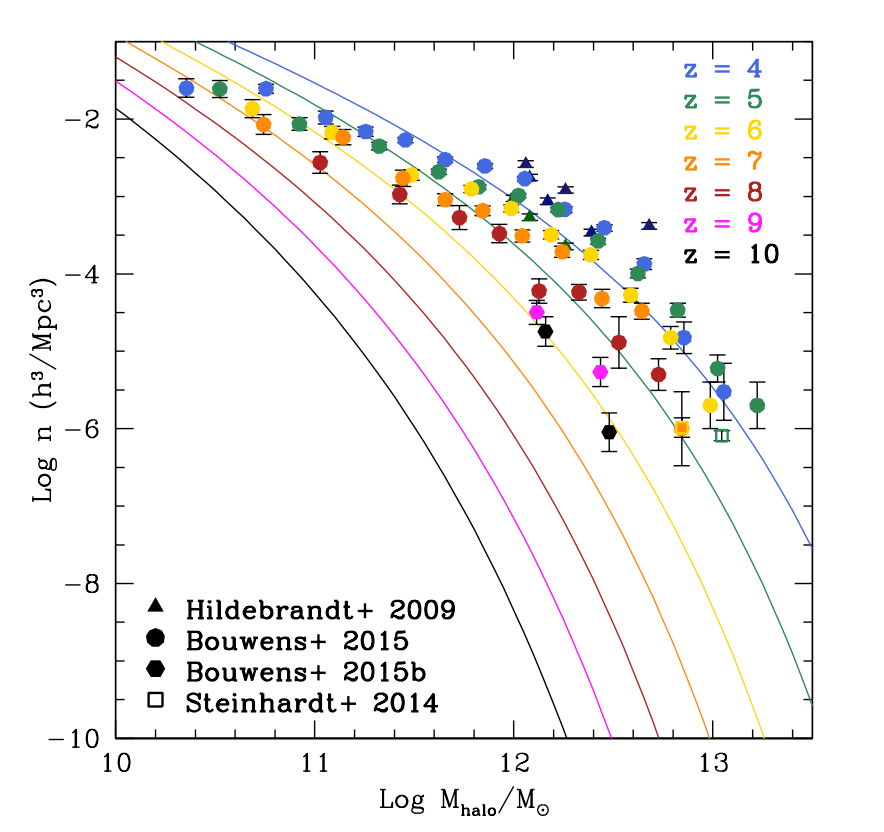
\includegraphics[scale=0.5]{Figures/steindhart_fig1}
		\caption{\label{fig:stein16_f1} Figura que representa la funci\'on de masa de halo. En l\'inea continua se muestra la predicci\'on te\'orica sacada de HMFCalc \citep{murray2013hmfcalc} y \cite{sheth2001ellipsoidal} mientr\'as que los marcadores muestran los valores obtenidos a trav\'es de las observaciones estudiadas en \cite{hildebrandt2009cars}, \cite{steinhardt2014uniform}, \cite{bouwens2015reionization} y \cite{bouwens2015uv}.}
		
	\end{center}
\end{figure}


El objetivo final de este trabajo pretende estudiar el problema IEGP desde tres enfoques distintos con la finalidad de clarificar cual puede ser el origen más plausible de las discrepancias observadas entre teoria y observaciones que parecen mostrar la \textbf{Figua \ref{fig:stein16_f1}}. Estos enfoque son:
\begin{description}
	\item[Observacional:] ¿Qué \textit{bias} observacionales pueden estar presentes? ¿Existen otros posibles \textit{bias} observacionales que no se hayan podido tomar en cuenta? ¿Hay otro tipos de sesgos que se hayan podido cometer al calcular la función de masa de halo de las observaciones consideradas? Desde esta perspectiva se pretenderá analizar el problema y determinar si tiene un papel relevante en la discrepancias observadas. También si nuevas observaciones y simulaciones contribuyen de manera positiva o negativa en este punto como por ejemplo los trabajos \cite{wang2019dominant} o \cite{behroozi2019universemachine}.
	
	\item[Física Bariónica:] Son muchos los trabajos que consideran que los procesos físicos de la matería bariónica podrían variar en función del redshift haciendo más eficiente, por ejemplo, los procesos de \textit{feedback} de AGNs que propicián la inhibición del SFR en redhift bajos \citep{finkelstein2015increasing}. Las recetas de la física bariónica juegan un papel fundamental en la relación entre masa estelar \textit{v.s} la masa del halo (SMHMR), veremos si son relevantes en este problema como parece plantear el trabajo de \cite{finkelstein2015increasing} o si por el contrario son suprimibles en el IEGP simplificando un poco el problema.
	
	\item[Modelo Cosmológico:] Por regla general y según ha marcado la experiencia de la historia científica, cuando existe una discrepancia entre observación y teoría suele ser el segundo factor el que está equivocado. Son muchos los logros del \lcdm pero también existen muchos problemas no explicados por este modelo y el IEGP parece convertirse en otro más. Daremos un repaso de los problemas que parece no explicar el \lcdm e intentaremos estudiar el IEGP considerando otros modelos cosmógicos y naturaleza de materia oscura que se encuentran sobre la mesa de teorías aceptadas o con el estatus de encontrase en consideración debido a las posibles carencias del \lcdm.
\end{description}


En esta primera sección daremos un pequeño resumen de los principales puntos del \textit{paper} de \cite{steinhardt2016impossibly} comparando de manera conjunta los resultados con los que se derivarían de las nuevas medidas ofrecidas por \cite{behroozi2019universemachine}, en un intento de ver si datos más actualizados pueden contribuir a solucionar o agravar las discrepancias observadas. En las siguientes secciones abordaremos de manera independiente los tres enfoques explicados terminando con una última sección dedicada a las conclusiones y a los posibles fututos trabajos que se podrían realizar en el campo de las simulaciones en aras de clarificar este problema . Pero lo primero es explicar el problema y allá vamos.


\section{\textit{The Impossible Early Galaxy Problem}.}

Existe un consenso bastante amplio en el que en un escenario basado en el modelo cosmológico \lcdm las grandes masas finales de los halos predichos por la función masa de halo cambian rápidamente entre los redshift 8 y 4, cuyos halos que contienen a las galaxias más masivas virializan hacia z=4 \citep{steinhardt2016impossibly}. Sin embargo, no se han encontrado evidencias de esa evolución esperada entre los rangos de redshift mencionados, por ejemplo, trabajos como el \cite{finkelstein2015increasing} y \cite{finkelstein2015evolution} han deducido una independencia del valor de la magnitud UV característica $M^*_{UV}$ de la función de  paraetrización de Scheter con respecto al redshift en los rangos z$\in [4,7]$, por tanto, sin encontrar signos de una evolución esperada entre las galaxias de estos redshift. Dichos trabajos encontraron un mayor número de galaxias brillantes en UV de lo esperado en redshift z=7 contrario a lo esperado y que concuerda con el resultado estudiado aquí del \textit{paper} de \cite{steinhardt2016impossibly} y que se puede visualizar en la \textbf{Figura \ref{fig:stein16_f1}}. En \cite{steinhardt2016impossibly} compara las funciones de masa de halo obtenidas de los trabajos de \cite{hildebrandt2009cars}, \cite{steinhardt2014uniform}, \cite{bouwens2015reionization} y \cite{bouwens2015uv} calculadas basándose en las observaciones de los estudios de CANDELS\footnote{\cite{grogin2011candels}}, CFHTLS\footnote{\cite{hildebrandt2009cars}} y SPLASH\footnote{\cite{capak2012splash}} y usando tres metodologías distintas que explicaremos en la siguiente subsección, con las funciones de masa de halo predichas por modelos teóricos obtenidos de la herramienta \textit{HMFCalc} \citep{murray2013hmfcalc} usando como base el trabajo de \cite{sheth2001ellipsoidal} y que explicaremos con un mayor detalle en otra subsección más adelante. Las discrepancias que se pueden observar en la \textbf{Figura \ref{fig:stein16_f1}} son muy notables y son estudiadas en \cite{steinhardt2016impossibly}. Aquí haremos un pequeño resumen de estas explicaciones aplicando las nuevas métricas obtenidas de \cite{behroozi2019universemachine} pero antes para poder comprender mejor los posibles \textit{bias} observacionales considerados u omitidos explicaremos en mayor detalle como se han obtenido dichas medidas de la función de masa de halo de las observaciones.

\section{Datos Observacionales}
Como ya se ha comentado, el trabajo de \cite{steinhardt2016impossibly} divide las estimaciones de la masa de halo de los diferentes campos observados en tres grupos según la técnica usada. Como se recalca en el \textit{paper} \cite{steinhardt2016impossibly} la ventaja de trabajar en redshifts altos es que nos permite ver diferentes fotogramas del universo con un intervalo más corto entre ellas que si la viésemos en rangos más bajos. En nuestro caso el rango medio del intervalo de tiempo entre los redshift 4 y 7 son de 0.9 giga-años, esto nos permite mediciones entre épocas más precisas aunque a cambio nos restringe bastante en los métodos disponibles para calcular la masa de halo de estos rangos, \cite{steinhardt2016impossibly} usa tres representados por diferentes \textit{papers}:
\begin{itemize}
	\item En el trabajo de \cite{hildebrandt2009cars} se muestra el método de clusterización, el cual estima la masa del halo según la distribución espacial de las galaxias. La ventaja de este método es que no hay que asumir ninguna propiedad físicas de las galaxias, pero sí es necesario escoger un modelo de materia oscura para las simulaciones.
	
	\item Un segundo método es el presentado y desarrollado en el artículo de \cite{finkelstein2015increasing}, el cual se basa en la curva de luminosidad UV y en la función de masa calculada a través de simulaciones de Bolshoi, relacionando ambas por el principio de que el halo más masivo a de albergar la galaxia más masiva y viceversa. Las mediciones plasmadas en la \textbf{Figura \ref{fig:stein16_f1}} de los estudios de \cite{bouwens2015reionization} y \cite{bouwens2015uv} usan esta técnica.
	
	\item El último método es asumir un ratio entre luminosidad/masa estelar y materia oscura. El ratio asumido es el redshift más bajos donde las estimaciones de materia oscura son más factibles por los métodos de agrupación. El ratio usado para el enlace entre masa estelar y de halo es $M_h/M_\star \sim 70 $ siendo la técnica usada en las mediciones de \cite{steinhardt2014uniform} que se presentan en la \textbf{Figura \ref{fig:stein16_f1}}.
\end{itemize}

Discutiremos estas tres técnicas por separado actualizando las medidas con los nuevos datos de \cite{behroozi2019universemachine}, pero antes de ello hagamos una pequeña presentación del trabajo de \cite{behroozi2019universemachine}.

\subsection{\textit{Universe Machine}}

En el trabajo de \cite{behroozi2019universemachine} se presenta uan serie de resultados derivados de la obtención de las estimaciones de la función de masa estelar, ratio de formación estelar cósmica y específica, la función de luminosidad UV, las fracciónes de amortiguamiento, funciones de autocorrelación, relación de masa estelar \textit{vs} UV y la relación IRX-UV determinadas a traves de simulaciones \textit{Marckov Chain Monte Carlo} (MCMC) usando los datos observacionales de los estudios de CANDELS, 3D-HST, ULTRAVISTA y ZFOURGE y las simulaciones de materia oscura de \textit{Bolshoi-Planck} y \textit{MDPL2}. Sin entrar en detalle en la explicación de la metodología (nos remitiremos a \cite{behroozi2019universemachine}) en el trabajo se presenta una serie de resultado de gran interés para el problema estudiado que intentaremos esbozar en las siguientes líneas:
\begin{description}
	\item[Relación masa estelar - UV] Las medidas dadas por \cite{bouwens2015reionization} y \cite{bouwens2015uv} representadas en la \textbf{Figura \ref{fig:stein16_f1}} están basadas en el trabajo de \cite{finkelstein2015increasing} el cual usa la relación entre masa estelar y masa de halo para lograr establecer una conexión entre la masa del halo y la luminosidad UV. En el trabajo de \cite{behroozi2019universemachine} se revisa la relación basándose en las distribuciones de probabilidad calculadas en las simulaciones MCMC de las funciones de masa estelar, luminosidad y las correcciones debidas a la atenuación de polvo según el redshift. Comparando los resultados de \cite{behroozi2019universemachine} con los de \cite{finkelstein2015increasing} encontramos que estos último se encuentran sobre-estimados con respecto a los últimos datos de los primeros (\textbf{Figura \ref{fig:cstm_behroozi_uvsm}}) en las galaxias más débiles, esto podría provocar una sobre-estimación de la masa de los halos ocasionando las discrepancias observadas.
	\begin{figure}[h]
		\begin{center}
			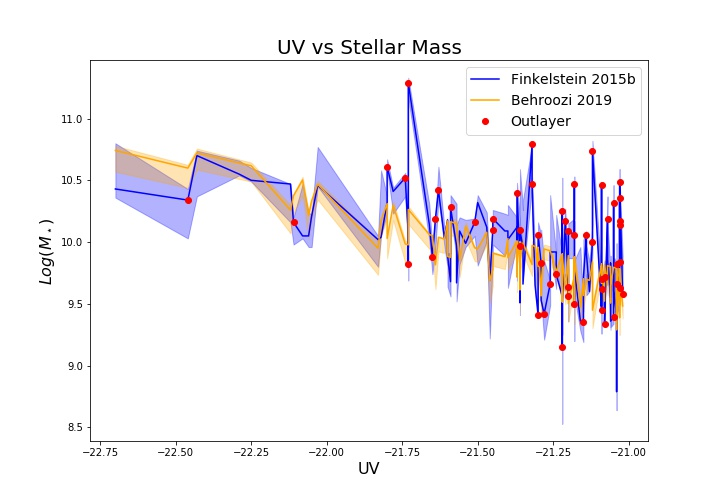
\includegraphics[scale=0.5]{Figures/behroozi_finkelstein_uvsm.jpg}
			\caption{\label{fig:cstm_behroozi_uvsm} En la figura se representa la función que relaciona la luminosidad UV y la masa estelar del trabajo de \cite{finkelstein2015increasing} \textit{vs} el resultado obtenido por el trabajo de \cite{behroozi2019universemachine}. Las observaciones son las usadas por \cite{finkelstein2015increasing} en el que representamos los intervalos de confianza de cada uno de los estudios. Hemos pintado en rojo aquellas mediciones de \cite{finkelstein2015increasing} que quedán fuera del intervalo de confianza de las mediciones de \cite{behroozi2019universemachine}. Se puede ver que principalmente se ven afectadas las galaxias menos brillantes de la muestra \textcolor{red}{sobre-estimando en general la masa estelar,} esto podría indicar que el ration SMHM puede ser menor intensificando el problema al contrario de lo que propone \cite{behroozi2019universemachine}.}
		\end{center}
	\end{figure}
	
	\item[Relación masa halo - masa estelar:] Uno de los resultados más interesantes según el interes de este trabajo es el estudio de la relación masa halo - masa estelar para el rango de redshift del estudio $z\in [0,10]$. Se encuentra que el ration SMHM varía entre galaxias satélite y galaxias centrales, por ejemplo en halos menos masivos le ratio de SMHM es mayor en las galaxias satélite ya que su tiempo de ``apagado''  es más largo creciendo en masa estelar mientras que permanece fija en su masa de materia oscura. Por otro lado en masas de halo altas el canal principal de crecimiento es via fusiones donde en las galaxias satélite es menos frecuente dando ratios de SMHM más bajos que en las galaxias centrales. La imagen del SMHM se complica en masas intermedias 
	
	
\end{description}

\subsection{Método de Clusterización}

\subsection{Método de función de luminosidad UV}

\subsection{Método de ratio luminosidad masa halo}

\section{Normalidad de las Galaxias}


%\include{Chapters/Chapter2} 
%\include{Chapters/Chapter3}
%\include{Chapters/Chapter4} 
%\include{Chapters/Chapter5} 

%----------------------------------------------------------------------------------------
%	BIBLIOGRAPHY
%----------------------------------------------------------------------------------------

\printbibliography[heading=bibintoc]

%----------------------------------------------------------------------------------------
%----------------------------------------------------------------------------------------
%	THESIS CONTENT - APPENDICES
%----------------------------------------------------------------------------------------

\appendix % Cue to tell LaTeX that the following "chapters" are Appendices

% Include the appendices of the thesis as separate files from the Appendices folder
% Uncomment the lines as you write the Appendices
% Chapter 1 v2

\chapter{Esquema} % Main chapter title

\label{indice} % For referencing the chapter elsewhere, use \ref{Chapter1} 


\section*{Planteamientos a contestar}
\begin{enumerate}
	\item \textbf{Introducción: Luces y sombras del modelo cosmológico estandar.}
	\begin{enumerate}[{1.}1]
		\item Modelo cosmológico estandar, breve descripción y principales logros.
		\item Naturaleza de la matería oscura, teorías y principales ventajas y desventajas de estás
		\item Evolución jerárquica de galaxias en la cosmología estandar.
		\begin{enumerate}[{1.3.}1]
			\item Descripción y teoría.
			\item Simulaciones.
			\item Predicciones, Problemas y Observaciones. Hasta que punto esos problemas se pueden solucionar en el modelo estándar.
		\end{enumerate}
		\item El papel actual de la física barionica como heroe al rescate a los problemas de la cosmología estándar.
		\item Papel de los modelos cosmológicos ante los mismos problemas y observaciones.
		\item ¿En qué punto nos encontramos?¿Por qué no encontramos candidatos a la CDM? Resumen.
	\end{enumerate}

	\item \textbf{Impossible Early Galaxy Problem.}
	\begin{enumerate}[{2.}1]
		\item Descripción del problema de \cite{steinhardt2016impossibly}.
		\begin{enumerate}[{2.1.}1]
			\item Plateamiento de las observaciones analizadas.
			\item Contexto teórico usado en la comparación, ¿es válido?
			\item Relación con otros problemas observados (Impossible Early Quasar Problem, Agujeros negros medianos)
		\end{enumerate}
		\item ¿Cómo abordamos el problema?
		\begin{enumerate}[{2.2.}1]
			\item Los tres posibles frentes: Observaciones mal interpretadas, Papel de la física Bariónica no considerado, Modelo Cosmológico fallido.
			\item Soluciones planteadas en \cite{steinhardt2016impossibly}.
			\item Soluciones de otros autores: Las observaciones están mal interpretadas \cite{behroozi2018mostmassive}, el modelo cosmológico es erroneo (Rh=c)...
			\item Otros trabajos que apoyan y rechazan las hipótesis de \cite{steinhardt2016impossibly}
		\end{enumerate}
	\end{enumerate}
	
	\item \textbf{Observaciones}
	\begin{enumerate}[{3.}1]
		\item Observaciones basadas en el ratio luminosidad - masa halo
		\begin{enumerate}[{3.1.}1]
			\item Descripción de las observaciones de \cite{bouwens2015uv}.
			\item Modelo usado por \cite{steinhardt2016impossibly} para la consversión luz-halo. Descripción del modelo \textit{abundance matching} que enlaza luminosidad con masa estelar. Consideración del enlace entre masa estelar y masa de halo por $M_\odot\sim 70 M\star$.
			\item Medidas de \citep{behroozi2019universemachine} y planteamiento de \cite{behroozi2018mostmassive} en el que plantea el error de \cite{steinhardt2016impossibly}. Análisis de ratio del ratio masa bariónica masa estelar. Rangos de error entre la relación SMHM. Método aplicado a las observaciones de \cite{bouwens2015uv}.
			\item Papel de nuevas observaciones en redhistf altos \citep{wang2019dominant}.
		\end{enumerate}
		\item Observaciones basadas en el \textit{cluster analysis}.
		\begin{enumerate}[{3.2.}1]
			\item Descripción de las observaciones de \cite{hildebrandt2009cars}. Resumen de la metodología.
			\item Posibles errores cometidos en la medida de estas y su incertidumbre.
			\item Dependencia del modelo cosmológico.
			\item Dependencia del volumen de galaxias observadas. ¿Qué pasa si existen muchas más galaxias de las consideradas?
		\end{enumerate}
		\item El papel de nuevas observaciones: \textit{JWST}
	\end{enumerate}
	
	\item \textbf{El papel de la Física Bariónica}
	\begin{enumerate}[{4.}1]
		\item Planteamientos de \cite{steinhardt2016impossibly} y efectos en las medidas.
		\item Una física variante puede implicar una evolución de los ratios de luminosidad, masa estelar y masa de halo.
		\item ¿Cómo considerar estos nuevos ingredientes? El papel de los modelos semi-analíticos
	\end{enumerate}
	
	\item \textbf{El modelo cosmológico}
	\begin{enumerate}[{5.}1]
		\item Descripción de la cosmología usada por \cite{steinhardt2016impossibly}.
		\item Resultados con la variación de parámetros usados.
		\item Simulaciones: Descripción delas Bolshoi y resultados con otras.
		\item ¿Qué pasaría si la teoría considerada no fuera correcta?
		\begin{enumerate}[{5.4.}1]
			\item Consideración de otra naturaleza de la materia oscura: WDM, FDM.
			\begin{enumerate}[{5.4.1.}1]
				\item Descripción
				\item Papel en la evolución galáctica
				\item Simulaciones y resultados
			\end{enumerate}
			\item Variaciones de la teoria: MOND, Rh=c,..
			\begin{enumerate}[{5.5.}1]
				\item Descripción
				\item Papel en la evolución galáctica
				\item Simulaciones y resultados
			\end{enumerate}
		\end{enumerate}
	\end{enumerate}
	
	\item \textbf{¿Y ahora qué? Como seguimos a partir de aquí.}
\end{enumerate}

\newpage
%% Appendix A

\chapter{Frequently Asked Questions} % Main appendix title

\label{AppendixA} % For referencing this appendix elsewhere, use \ref{AppendixA}

\section{How do I change the colors of links?}

The color of links can be changed to your liking using:

{\small\verb!\hypersetup{urlcolor=red}!}, or

{\small\verb!\hypersetup{citecolor=green}!}, or

{\small\verb!\hypersetup{allcolor=blue}!}.

\noindent If you want to completely hide the links, you can use:

{\small\verb!\hypersetup{allcolors=.}!}, or even better: 

{\small\verb!\hypersetup{hidelinks}!}.

\noindent If you want to have obvious links in the PDF but not the printed text, use:

{\small\verb!\hypersetup{colorlinks=false}!}.

%\include{Appendices/AppendixB}
%\include{Appendices/AppendixC}


\end{document}  
